% !TeX root = skripta-konstitutivni-vztahy.tex
% !TeX lastmodified = 2016-11-01

\subsection{Model Mooney-Rivlin}\label{sec:mooney-rivlin}
\subsubsection{Mooneyho formulace (1940)}\label{subsec:mooneyho-formulace}
\begin{itemize}
	\item guma je nestlačitelná a izotropní v nedeformovaném stavu
	\item Hookeův zákon platí pro „simple shear“ nebo „simple shear“ s~kombinací předchozího tlaku nebo tahu (simple shear v rovině kolmé na předchozí zatížení) 
\end{itemize}

Čistě matematická formulace hustoty deformační energie ve tvaru:
\begin{equation}
	W = C_1  \left(\lambda_1^2 + \lambda_2^2 + \lambda_3^2 - 3\right) + C_2 \left(\frac{1}{\lambda_1^2} + \frac{1}{\lambda_1^2} + \frac{1}{\lambda_1^2} - 3\right),
\end{equation}
kde $C_1 [\si{\mega\pascal}]$ a~$C_2 [\si{\mega\pascal}]$ jsou materiálové parametry.

Pokud $C_2 = 0$, pak existuje zřejmá podobnost s~modelem Neo-Hook
\begin{equation}
	2 C_1 = G = N k T,
\end{equation}
kde
\begin{itemize}
	\item[$N$] je počet řetězců v~objemu,
	\item[$k$] je Boltzmanova konstanta,
	\item[$T$] je termodynamická teplota.
\end{itemize}

\begin{figure}[H]
	\centering
	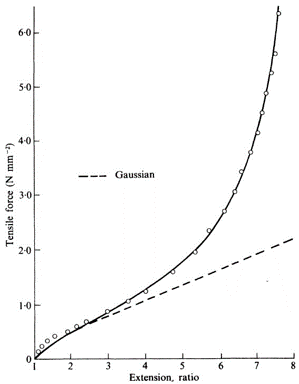
\includegraphics[height=6cm]{mooneyho-formulace}
	\caption{Aproximace experimentu Mooneyho formulací}
	\label{fig:mooneyho-formulace}
\end{figure}

\subsubsection{Rivlinova formulace (1948)}\label{subsec:rivlinova-formulace}
\begin{itemize}
	\item guma je nestlačitelná a~izotropní v~nedeformovaném stavu
	\item + logický závěr: pokud je materiál izotropní, funkce deformační energie by měla být symetrická s~ohledem na $\lambda_1$, $\lambda_2$, $\lambda_3$
	\item navrženou $W$ nesmí ovlivnit změna znaménka u~dvou $\lambda_i$ (souvisí s~rotací tělesa o~$\SI{180}{\degree}$)
\end{itemize}

Navržená $W$ by tedy měla být konvexní (polykonvexní), Rivlin navrhuje „strain ellipsoid“
\begin{itemize}
	\item Existence globálního minima energie
	\item Kladný přírůstek napětí při kladném přírůstku deformace
\end{itemize}

Pak lze zřejmě vytvořit určité vztahy, tj. invaritanty, pro $\lambda_i$.
Rivlin je navrhuje, ve formě druhých mocnin následovně:
\begin{equation}\begin{split}
	I_1 &= \lambda_1^2 + \lambda_2^2 + \lambda_3^2\\
	I_2 &= \lambda_1^2 \lambda_2^2 + \lambda_2^2 \lambda_3^2 + \lambda_3^2 \lambda_1^2\\
	I_3 &= \lambda_1^2 \lambda_2^2 \lambda_3^2
\end{split}\end{equation}

\begin{figure}[H]
	\centering
	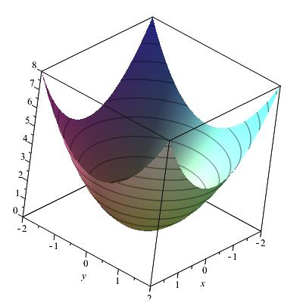
\includegraphics{rivlinova-formulace}
	\caption{Konvexní funkce}
	\label{fig:rivlinova-formulace}
\end{figure}

Nestlačitelnost umožňuje definovat předchozí dva invarianty jako:
\begin{equation}\begin{split}
	I_1 &= \lambda_1^2 + \lambda_2^2 + \lambda_3^2\\
	I_2 &= \lambda_1^2 \lambda_2^2 + \lambda_2^2 \lambda_3^2 + \lambda_3^2 \lambda_1^2 = \frac{1}{\lambda_1^2} + \frac{1}{\lambda_2^2} + \frac{1}{\lambda_3^2}
\end{split}\end{equation}

V~podobě dvou nezávislých invariantů je tak navržena i~energie napjatosti
\begin{equation}
	W = \sum\limits_{i=0, j=0}^{\infty} C_{ij} (I_1-3)^i (I_2-3)^j,
\end{equation}
přičemž $(I_1-3)$ a~$(I_2-3)$ je navrženo schválně, aby členy byly $0$ při nulových deformacích a~$C_{\infty}=0$ ze stejného důvodu.

Bohužel, bez nějaké „první“ znalosti o~křivce $\sigma-\varepsilon$ je velmi obtížné vybrat koeficienty $i$,$j$ smysluplně. Většinou se berou první členy rozvoje.

\begin{equation}\begin{split}
	i=1, j=0: \quad &W = C_{10} (I_1-3)^1 = C_{10} \left(\lambda_1^2 + \lambda_2^2 + \lambda_3^2 - 3\right) \quad \text{\ldots Neo-Hook}\\
	i=0, j=1: \quad &W = C_{01} (I_2-3)^1 = C_{01} \left(\frac{1}{\lambda_1^2} + \frac{1}{\lambda_2^2} + \frac{1}{\lambda_3^2} - 3\right) \quad \text{\ldots nemá aplikaci}
\end{split}\end{equation}
Kombinace obou dává opět \hyperref[subsec:mooneyho-formulace]{Mooneyho formulaci}. Co další kombinace?
